\documentclass{beamer}
\usetheme{Warsaw}
\usepackage[utf8]{inputenc}
\usepackage[T1]{fontenc}
\usepackage[french]{babel}
\usepackage{amsmath, amssymb}
\usepackage{graphicx}
\usepackage{pgfplots}
\pgfplotsset{compat=1.18}
\usepackage{listings}
\usepackage{xcolor}
\usepackage{algorithm}
\usepackage{algorithmic}
\usepackage{url}
\usepackage{tikz}
\usetikzlibrary{trees,positioning,shapes}
%\usepackage{pgfpages}


%\setbeameroption{show notes on second screen=right} % Both

% Configuration pour les listings de code
\lstset{
	language=C++,
	basicstyle=\tiny\ttfamily,
	keywordstyle=\color{blue},
	commentstyle=\color{green!50!black},
	stringstyle=\color{red},
	numbers=left,
	numberstyle=\tiny,
	stepnumber=1,
	numbersep=5pt,
	backgroundcolor=\color{gray!10},
	frame=single,
	breaklines=true,
	breakatwhitespace=true,
	tabsize=2
}

\title{Parallélisme du Random Forest}
\subtitle{Machine Learning}
\titlegraphic{
\includegraphics[height=1.5cm]{assets/imsp.png}}
\author[Béryl]{Béryl HOUESSOU}
\institute{Institut de Mathématiques et de Sciences Physiques\\
	Université d'Abomey-Calavi, Bénin}
\date{\today}


\begin{document}
	
	%-------------------------
	\begin{frame}
		\titlepage
		\note{Bonjour à tous, mon thème de présentation porte sur le Parallélisme du Random Forest. Mais avant tout propos, permettez-moi cette question.}
	\end{frame}
	
	%-------------------------
	\begin{frame}{Introduction}
		\begin{center}
			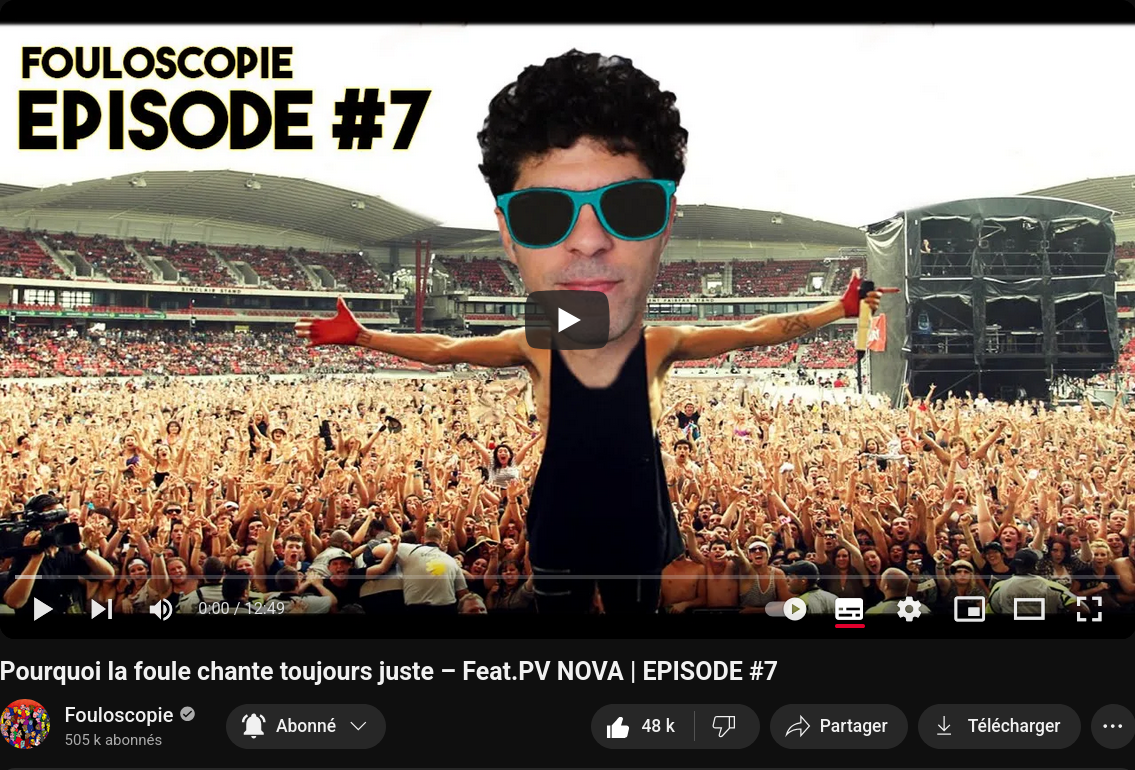
\includegraphics[width=0.6\textwidth]{assets/Pourquoi_la_foule_chante_toujours_juste.png}
			
			\vspace{0.5cm}
			{\Large \textbf{Pourquoi lors des concerts, la foule chante-t-elle toujours juste ?}}
		\end{center}
		\note{
	Individuellement, chaque chanteur amateur fait des erreurs, mais collectivement la voix de la foule est toujours juste. En effet, la foule est composée de plusieurs voix qui s'additionnent et se corrigent mutuellement.
	Cela peut sembler éloigné du machine learning, mais ce phénomène d'intelligence collective est au cœur des models ensemblistes, comme le Random Forest. Dans ces modèles, plusieurs arbres de décision sont construits et leurs résultats sont combinés pour obtenir une prédiction plus précise. Ici, chaque arbre peut être vu comme un chanteur amateur, et la forêt comme la foule qui chante juste.
}
	\end{frame}
	
	%-------------------------
	\begin{frame}{De la foule au Random Forest}
		\begin{columns}
			\begin{column}{0.5\textwidth}
				\textbf{Dans un concert :}
				\begin{itemize}
					\item<1-> Chaque chanteur fait des erreurs
					\item<2-> Collectivement : voix juste
					\item<3-> Correction mutuelle
				\end{itemize}
			\end{column}
			\begin{column}{0.5\textwidth}
				\textbf{Dans Random Forest :}
				\begin{itemize}
					\item<1-> Chaque arbre fait des erreurs
					\item<2-> Collectivement : prédiction plus ou moins précise
					\item<3-> Agrégation des résultats
				\end{itemize}
			\end{column}
		\end{columns}
		
		\vspace{0.5cm}
		\begin{center}
			\onslide<4->{\textcolor{blue}{\textbf{Intelligence collective = Modèles ensemblistes}}}
		\end{center}
		\note{Individuellement, chaque chanteur amateur fait des erreurs, mais collectivement la voix de la foule est toujours juste. Dans les modèles ensemblistes comme Random Forest, chaque arbre peut être vu comme un chanteur amateur, et la forêt comme la foule qui chante juste.}
	\end{frame}
	
	%-------------------------
	\begin{frame}{Qu'est-ce que le Random Forest ?}
		\begin{block}{Définition}
			Algorithme d'apprentissage automatique ensembliste qui :
			\begin{itemize}
				\item<1-> Construit plusieurs arbres sur des \textbf{échantillons aléatoires}
				\item<2-> \textbf{Combine leurs résultats} pour une prédiction finale
				\item<3-> Réduit le surapprentissage et améliore la robustesse
			\end{itemize}
		\end{block}
		
		\begin{center}
			\onslide<4->{
				\begin{tikzpicture}[scale=0.8]
					% Données d'entrée
					\node[draw, rectangle] at (0,0) {Données};
					
					% Arbres
					\foreach \i in {1,2,3} {
						\node[draw, circle] at (2*\i, -1) {$T_{\i}$};
						\draw[->] (0,0) -- (2*\i, -1);
					}
					
					% Agrégation
					\node[draw, rectangle] at (4, -2.5) {Agrégation};
					\foreach \i in {1,2,3} {
						\draw[->] (2*\i, -1) -- (4, -2.5);
					}
					
					% Prédiction finale
					\node[draw, rectangle, fill=green!20] at (4, -4) {Prédiction};
					\draw[->] (4, -2.5) -- (4, -4);
				\end{tikzpicture}
			}
		\end{center}
		\note{Le Random Forest utilise une approche ensembliste pour améliorer la précision des prédictions. Cette méthode permet de réduire le risque de surapprentissage.}
	\end{frame}
	
	%-------------------------
	\begin{frame}{Algorithme Random Forest}
		\onslide{
			\begin{algorithm}[H]
				\caption{Random Forest}
				\begin{algorithmic}[1]
					\REQUIRE Ensemble d'entraînement $D$, nombre d'arbres $n$
					\ENSURE Forêt de décision $F$
					\STATE Initialiser $F \gets \emptyset$
					\FOR{$i = 1$ à $n$}
					\STATE $D_i \gets$ échantillon bootstrap de $D$
					\STATE $T_i \gets$ construire un arbre de décision sur $D_i$
					\STATE Ajouter $T_i$ à $F$
					\ENDFOR
					\RETURN $F$
				\end{algorithmic}
			\end{algorithm}
		}
		\note{Voici l'algorithme de base du Random Forest. Chaque arbre est construit sur un échantillon bootstrap différent.}
	\end{frame}
	
	%-------------------------
	\begin{frame}{Construction des arbres : Bagging}
		\begin{block}{Bootstrap Aggregating}
			\textbf{Principe :} Créer plusieurs sous-ensembles par échantillonnage avec remise
		\end{block}
		
		\begin{center}
			\onslide<2->{
				\begin{tikzpicture}[scale=0.7]
					% Dataset original
					\node[draw, rectangle, minimum width=2cm] at (0,2) {Dataset $D$};
					
					% Bootstrap samples
					\foreach \i in {1,2,3} {
						\node[draw, rectangle, fill=blue!20] at (3*\i-1, 0) {$D_{\i}$};
						\draw[->] (0,2) -- (3*\i-1, 0);
						\node[below] at (3*\i-1, -0.5) {Bootstrap};
					}
					
					% Arbres
					\foreach \i in {1,2,3} {
						\node[draw, circle, fill=green!20] at (3*\i-1, -2) {$T_{\i}$};
						\draw[->] (3*\i-1, 0) -- (3*\i-1, -2);
					}
				\end{tikzpicture}
			}
		\end{center}
		
		\onslide<3->{\textbf{Avantage :} Rajouter de la diversité entre les arbres, ce qui réduit le surapprentissage et améliore la généralisation.}
		\note{Le bagging consiste à créer plusieurs sous-ensembles de données à partir de l'ensemble d'entraînement initial. Cette approche permet d'amener de la diversité entre les arbres, ce qui réduit le surapprentissage et améliore la généralisation. Aussi les modèles d'arbres de décision étant déterministes c'est-à-dire qu'avec les mêmes données d'entraînement j'obtiens toujours les mêmes arbres, le bagging permet d'atténuer cet effet en introduisant de la variabilité.}
	\end{frame}
	
	%-------------------------
	\begin{frame}{Mesures de pureté}
		\begin{columns}
			\begin{column}{0.5\textwidth}
				\onslide<1->{\textbf{Entropie}}
				\onslide<2->{$$H(X) = -\sum_{i=1}^{n} p_i \log_2(p_i)$$}
				\begin{itemize}
					\item<3-> Varie entre 0 et 1
					\item<4-> 0 = distribution homogène
					\item<5-> 1 = distribution hétérogène
				\end{itemize}
			\end{column}
			\begin{column}{0.5\textwidth}
				\onslide<6->{\textbf{Indice de Gini}}
				\onslide<7->{$$Gini(X) = 1 - \sum_{i=1}^{n} p_i^2$$}
				\begin{itemize}
					\item<8-> Varie entre 0 et 0,5
					\item<9-> 0 = pureté parfaite
					\item<10-> 0,5 = désordre maximal
				\end{itemize}
			\end{column}
		\end{columns}
		\note{Pour choisir les variables à chaque nœud, on utilise une mesure de qualité comme l'entropie ou l'indice de Gini. L'objectif est de maximiser la pureté des nœuds.}
	\end{frame}
	
	%-------------------------
	\begin{frame}{Construction d'un arbre}
		\begin{algorithm}[H]
			\caption{Construction d'un arbre de décision}
			\begin{algorithmic}[1]
				\REQUIRE Ensemble $D$, profondeur max $d$, échantillons min $m$
				\ENSURE Arbre de décision $T$
				\IF{profondeur max atteinte OU $|D| < m$}
				\RETURN feuille (classe majoritaire/moyenne)
				\ENDIF
				\STATE Sélectionner sous-ensemble aléatoire de caractéristiques
				\FOR{chaque caractéristique}
				\STATE Calculer gain d'impureté pour chaque seuil
				\ENDFOR
				\STATE Choisir meilleure caractéristique et seuil
				\STATE Créer $D_{gauche}$ et $D_{droite}$
				\STATE $T_{gauche} \gets$ récursion sur $D_{gauche}$
				\STATE $T_{droite} \gets$ récursion sur $D_{droite}$
				\RETURN $T$
			\end{algorithmic}
		\end{algorithm}
		\note{Voici l'algorithme de construction d'un arbre dans le contexte du Random Forest. Une petite piqure de rappel : Un arbre de décision est un modèle d'apprentissage supervisé qui se construit selon un processus récursif de partitionnement des données. On commence par un nœud racine représentant l'ensemble complet des données, puis on divise cet ensemble en sous-ensembles plus petits, de manière à rendre ces groupes aussi homogènes que possible par rapport à la variable cible. Suivant cette logique, il nous faut trouver des critères d'arrêt pour notre algo de construction d'arbre (étant récursif) donc ici nous avons la profondeur maximale et le nombre minimum d'échantillons par feuille. Ces deux critères sont importants pour éviter le surapprentissage, parce qu'on ne veut pas que l'arbre devienne trop complexe et s'adapte trop aux données d'entraînement, ce qui pourrait nuire à sa capacité de généralisation.}
	\end{frame}
	
	%-------------------------
	\begin{frame}{Sélection aléatoire de caractéristiques: Feature bagging}
		\begin{block}{Objectif}
			Réduire la corrélation entre arbres et améliorer la diversité
		\end{block}
		
		\begin{center}
			\begin{tikzpicture}[scale=0.8]
				% Caractéristiques disponibles
				\node[draw, rectangle] at (0,2) {Features: $\{f_1, f_2, f_3, f_4, f_5\}$};
				
				% Sélection aléatoire pour chaque nœud
				\foreach \i in {1,2,3} {
					\node[draw, rectangle, fill=orange!20] at (3*\i-1, 0) {$\{f_{\i}, f_{\i+1}\}$};
					\draw[->] (0,2) -- (3*\i-1, 0);
					\node[below] at (3*\i-1, -0.5) {Nœud \i};
				}
			\end{tikzpicture}
		\end{center}
		
		\textbf{Avantages :}
		\begin{itemize}
			\item Évite la domination par quelques caractéristiques
			\item Particulièrement utile avec beaucoup de features
		\end{itemize}
		\note{À chaque nœud de l'arbre, un sous-ensemble aléatoire de caractéristiques est sélectionné. Cela permet de réduire la corrélation entre les arbres et améliore la qualité globale des prédictions.}
	\end{frame}
	
	%-------------------------
	\begin{frame}{Agrégation des résultats}
		\begin{columns}
			\begin{column}{0.5\textwidth}
				\textbf{Classification}
				\begin{itemize}
					\item Vote majoritaire
					\item Classe la plus fréquente
				\end{itemize}
				
				\vspace{1cm}
				\begin{tikzpicture}[scale=0.6]
					\node at (0,2) {$T_1$: A};
					\node at (0,1) {$T_2$: B};
					\node at (0,0) {$T_3$: A};
					\node[draw, fill=green!20] at (3,1) {Résultat: A};
					\draw[->] (0.5,1) -- (2.5,1);
				\end{tikzpicture}
			\end{column}
			\begin{column}{0.5\textwidth}
				\textbf{Régression}
				\begin{itemize}
					\item Moyenne des prédictions
					\item Réduction de la variance
				\end{itemize}
				
				\vspace{1cm}
				\begin{tikzpicture}[scale=0.6]
					\node at (0,2) {$T_1$: 5.2};
					\node at (0,1) {$T_2$: 4.8};
					\node at (0,0) {$T_3$: 5.1};
					\node[draw, fill=green!20] at (4,1) {Résultat: 5.03};
					\draw[->] (0.5,1) -- (3.5,1);
				\end{tikzpicture}
			\end{column}
		\end{columns}
		\note{L'agrégation est la dernière étape du Random Forest. Elle combine les prédictions de tous les arbres pour obtenir une prédiction finale plus robuste.}
	\end{frame}
	
	%-------------------------
	\begin{frame}{Avantages et inconvénients du Random Forest}
		\begin{columns}
			\begin{column}{0.5\textwidth}
				\onslide<1->{\textbf{Avantages}}
				\begin{itemize}
					\item<1-> \textbf{Robustesse :} Réduit le surapprentissage
					\item<1-> \textbf{Précision :} Souvent supérieure aux arbres individuels
					\item<1-> \textbf{Versatilité :} Fonctionne sur différents types de données
					\item<1-> \textbf{Gestion du bruit :} Résistant aux données aberrantes
					\item<1-> \textbf{Pas de normalisation :} Invariant aux transformations monotones
				\end{itemize}
			\end{column}
			\begin{column}{0.5\textwidth}
				\onslide<2->{\textbf{Inconvénients}}
				\begin{itemize}
					\item<2-> \textbf{Coût computationnel :} Temps de calcul élevé
					\item<2-> \textbf{Mémoire :} Consommation importante
					\item<2-> \textbf{Interprétabilité :} Moins lisible qu'un arbre unique
					\item<2-> \textbf{Surapprentissage :} Possible avec trop d'arbres
					\item<2-> \textbf{Biais :} Peut favoriser les features avec plus de modalités
				\end{itemize}
			\end{column}
		\end{columns}
		
		\vspace{0.5cm}
		\begin{center}
			\onslide<3->{\textcolor{red}{\textbf{Solution aux problèmes de performance : La parallélisation !}}}
		\end{center}
		\note{Le Random Forest présente plusieurs avantages qui en font un algorithme populaire : robustesse, précision, versatilité. Toutefois, il n'est pas sans défauts, notamment en termes de coût computationnel. C'est là que la parallélisation entre en jeu.}
	\end{frame}
	
	%-------------------------
	\begin{frame}{Parallélisation : Pourquoi ?}
		\begin{block}{Limitations du Random Forest}
			\begin{itemize}
				\item<1-> Coûteux en temps de calcul
				\item<1-> Consommation mémoire importante
				\item<1-> Lent avec beaucoup d'arbres
			\end{itemize}
		\end{block}
		
		\begin{block}{Avantages de la parallélisation}
			\begin{itemize}
				\item<2-> \textbf{Efficacité :} Réduit le temps d'entraînement
				\item<2-> \textbf{Scalabilité :} Gère de gros volumes de données
				\item<2-> \textbf{Indépendance :} Chaque arbre peut être construit séparément
			\end{itemize}
		\end{block}
		\note{Le Random Forest n'est pas sans défauts. Il peut être coûteux en termes de temps de calcul et de mémoire. C'est là que la parallélisation entre en jeu.}
	\end{frame}
	
	%-------------------------
	\begin{frame}{Thread vs Processus}
		\begin{center}
			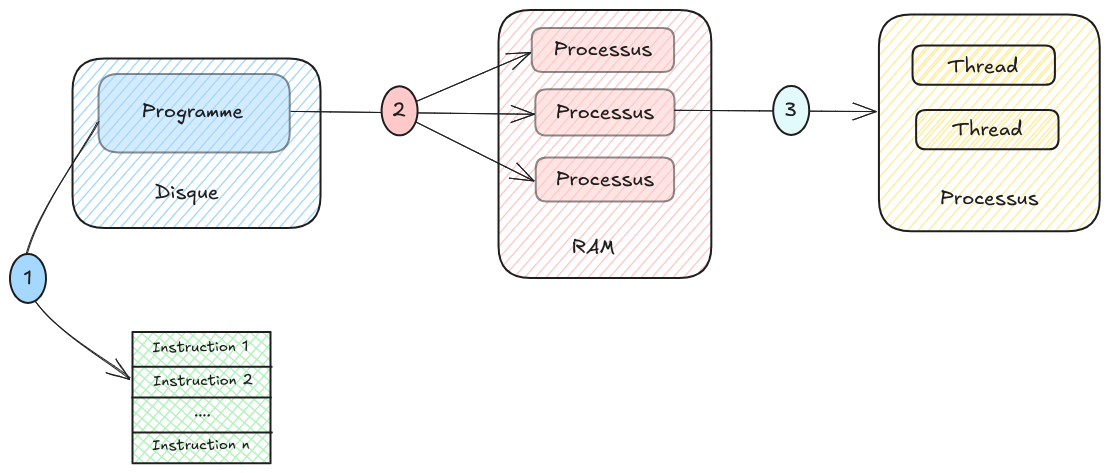
\includegraphics[width=0.8\textwidth]{assets/process_thread.png}
		\end{center}
		
		\begin{block}{Thread}
			\begin{itemize}
				\item<2-> Unité d'exécution indépendante dans un processus
				\item<3-> Partage mémoire et ressources
				\item<4-> Communication rapide mais synchronisation nécessaire
			\end{itemize}
		\end{block}
		\note{Un thread est une unité d'exécution indépendante au sein d'un processus. 
    Un processus peut donc contenir plusieurs threads, chacun exécutant une tâche spécifique.
    UN processus étant un programme en cours d'exécution, il peut contenir plusieurs threads qui partagent la même mémoire et les mêmes ressources.}
	\end{frame}
	
	%-------------------------
	\begin{frame}[fragile]{Parallélisation avec std::thread}
		\begin{lstlisting}[basicstyle=\scriptsize\ttfamily]
	#include <vector>
	#include <thread>
	
	void build_tree_for_index(int i, std::vector<Tree>& trees, 
	const std::vector<Data>& data_samples) {
		trees[i] = build_tree(data_samples[i]);
	}
	
	void build_forest_parallel(std::vector<Tree>& trees, 
	const std::vector<Data>& data_samples) {
		std::vector<std::thread> threads;
		int n_trees = trees.size();
		
		// Creation des threads
		for (int i = 0; i < n_trees; ++i) {
			threads.emplace_back(build_tree_for_index, i, 
			std::ref(trees), std::cref(data_samples));
		}
		
		// Synchronisation
		for (auto& t : threads) t.join();
	}
		\end{lstlisting}
		\note{
\texttt{threads.emplace\_back(...)} ajoute un nouvel élément à la fin du vecteur \texttt{threads}. \texttt{emplace\_back} construit un nouvel objet directement dans la mémoire du vecteur, évitant la création d'un objet temporaire. 
Les arguments passés à \texttt{emplace\_back} sont utilisés pour construire le nouveau \texttt{std::thread}.
Le premier, \texttt{build\_tree\_for\_index}, est la fonction que ce nouveau thread exécutera. 
Les autres sont ceux qui seront passés à cette dernière lorsque le thread démarrera.
  \begin{itemize}
    \item \texttt{i} : l'index de l'arbre à construit dans le vecteur trees.
    \item \texttt{std::ref(trees)} : Le constructeur \texttt{std::thread} copie par défaut ses arguments. \texttt{std::ref} est un wrapper qui garantit que l'objet \texttt{trees} est passé \textbf{par référence}. Cela signifie que la fonction du thread peut accéder directement au conteneur \texttt{trees} d'origine et le modifier, plutôt qu'à une copie. Cela est essentiel car la tâche du thread consiste à ajouter un nouvel arbre à ce conteneur partagé.
    \item \texttt{std::cref(data\_samples)} : similaire à \texttt{std::ref}, \texttt{std::cref} transmet l'objet \texttt{data\_samples} \textbf{par référence constante}. L'aspect \texttt{const} garantit que le thread ne peut pas modifier les données d'entrée d'origine.
  \end{itemize}
}
	\end{frame}
	
	%-------------------------
	\begin{frame}{Étapes de la parallélisation}
		\begin{enumerate}
			\item<1-> \textbf{Création des threads}
			\begin{itemize}
				\item<1-> Un thread par arbre à construire
				\item<1-> Fonction de construction + données bootstrap
			\end{itemize}
			
			\item<2-> \textbf{Synchronisation}
			\begin{itemize}
				\item<2-> Attendre tous les threads (\texttt{join()})
			\end{itemize}
			
			\item<3-> \textbf{Gestion des résultats}
			\begin{itemize}
				  \item<3-> Chaque thread écrit dans une zone mémoire distincte
				  \item<3-> Pas de partage de données modifiables
				\end{itemize}
		\end{enumerate}
		
		\note{Voici comment procéder pour la parallélisation : création des threads, synchronisation et gestion des résultats. Il est important de s'assurer que chaque thread écrit dans une zone mémoire distincte.}
	\end{frame}
	
	%-------------------------
	\begin{frame}{Exercice pratique : Reconnaissance des chiffres}
		\begin{columns}
			\begin{column}{0.6\textwidth}
				\textbf{Problème :} Reconnaître les chiffres 0-9 à partir de 7 segments
				
				\begin{center}
					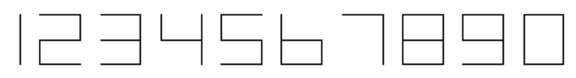
\includegraphics[width=0.8\textwidth]{assets/digits.png}
				\end{center}
				
				\textbf{Représentation :}
				\begin{itemize}
					\item Vecteur binaire de 7 éléments
					\item 1 = segment allumé, 0 = éteint
					\item Exemple : "8" = [1,1,1,1,1,1,1]
				\end{itemize}
			\end{column}
			\begin{column}{0.4\textwidth}
				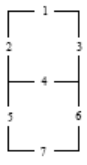
\includegraphics[width=\textwidth]{assets/digits_segment.png}
				
				\vspace{0.5cm}
				\textbf{Application RF :}
				\begin{itemize}
					\item 7 features binaires
					\item 10 classes (0-9)
					\item Parallélisation des arbres
				\end{itemize}
			\end{column}
		\end{columns}
		\note{Dans cet exercice pratique, nous avons 10 chiffres représentés par des combinaisons de 7 segments lumineux. Chaque chiffre est un vecteur binaire de 7 dimensions.}
	\end{frame}
	
	%-------------------------
	\begin{frame}{Conclusion}
		\begin{block}{Points clés}
			\begin{itemize}
				\item<1-> \textbf{Random Forest :} Intelligence collective appliquée au ML
				\item<1-> \textbf{Robustesse :} Réduction du surapprentissage par agrégation
				\item<1-> \textbf{Parallélisation :} Accélération grâce à l'indépendance des arbres
			\end{itemize}
		\end{block}
		
		\begin{block}{Perspectives}<2->
			\begin{itemize}
				\item<2-> Autres algorithmes ensemblistes (XGBoost, LightGBM)
			\end{itemize}
		\end{block}
		\note{En conclusion, le Random Forest est un algorithme puissant qui utilise l'intelligence collective pour améliorer les prédictions. Sa parallélisation permet d'exploiter efficacement les ressources matérielles modernes.}
	\end{frame}
	
	%-------------------------
	\begin{frame}{Merci, pour votre attention !}
		\begin{center}
			
\includegraphics[width=0.5\textwidth]{assets/thank-35.png}
		\end{center}
	\end{frame}
	
\end{document}